%\documentclass[draft]{ws-procs11x85}
%\documentclass[square]{ws-procs11x85}
\documentclass{ws-procs11x85}
\usepackage{color}
\usepackage{graphicx}
\usepackage{subfigure}
\usepackage{wrapfig}
\usepackage{multirow}
\usepackage{url}
\usepackage{titlesec}
\usepackage{wrapfig}
\usepackage{algorithm}
\usepackage{algorithmic}


\titlespacing{\section}{0pt}{1mm}{1mm}
\titlespacing{\subsection}{0pt}{0.5mm}{0.5mm}
\titlespacing{\subsubsection}{0pt}{0.8mm}{0.8mm}


\setlength{\textheight}{22.6cm}  % Tamer
\setlength{\textwidth}{17.2cm}   %Tamer

\setlength\oddsidemargin{1.75cm}   % Tamer
\setlength\evensidemargin{1.75cm}   % Tamer




\newcommand{\tk}[1]{{\bf {\textcolor{magenta}{#1 -- TK}}}}

\newcommand{\hg}[1]{{\bf {\textcolor{red}{#1 -- HG}}}}

\newtheorem{define}{Definition}
\renewcommand{\baselinestretch}{0.98}

\long\def \ignoreme#1{}
\newcommand{\goodgap}{
        \hspace{\subfigtopskip}
        \hspace{\subfigbottomskip}
}


\begin{document}


\noindent
\centerline{\LARGE \bf Cover Letter}\\

\noindent {\bf Paper Title:}\\
ENHANCED COLOR CODING FOR SIGNALING PATHWAY DETECTION IN PROTEIN
INTERACTION NETWORKS\\

\noindent
{\bf Contact Author:} \\
{\bf Name:} Tamer Kahveci\\
{\bf Email:} tamer@cise.ufl.edu\\

\noindent
{\bf PSB Session:}\\
Identification of Aberrant Pathway and Network Activity from High-Throughput Data

\begin{center}
 The submitted paper contains original, unpublished results, and is
 not currently under consideration elsewhere.  All co-authors concur
 with the contents of the paper.
\end{center}

%\thispagestyle{empty}
\pagebreak
\addtocounter{page}{-1}

%\pagestyle{plain}



\title{ENHANCED COLOR CODING FOR SIGNALING PATHWAY DETECTION IN PROTEIN
INTERACTION NETWORKS}

\author{Haitham Gabr, Alin Dobra and Tamer Kahveci$^*$}

\address{CISE Department, University of Florida,\\
Gainesville, FL 32611, USA\\
E-mail: \{hgabr, adobra, tamer$^*$\}@cise.ufl.edu}

\begin{abstract} 
	Discovering signaling pathways in protein interaction networks is a key
	ingredient for understanding how proteins carry out cellular function. Among
	the outstanding techniques that have been recently used in pathway detection and
	other related problems is color coding. This technique allows for faster
	detection of signaling pathways, but still has a very good potential of
	enhancement. We present an enhancement to color coding, which can be applied
	to virtually any method that uses it. We use the enhanced color coding
	technique to find signaling pathways in protein interaction networks. We show
	that our method takes less time than the leading one to find the same results.
	We also validate our method by testing the statistical and biological
	significance of the results.
\end{abstract}

\keywords{protein interaction networks; signaling pathways; color coding;
chromatic polynomial}

\bodymatter

\section{Introduction} 
\label{introduction}

\ignoreme{
\hg{ read carefully and fix any typo, grammatical error, logical error
  etc}

\hg {see where we can cut about 1 page}

\hg{ write short abstract + very short conclusion. You can copy paste
  from intro. Abstract is in present tense. Conclusion in past tense.}
}

Studying interactions between proteins has been of utmost importance
in understanding how proteins work collectively to govern cellular
function~\cite{schwikowski,uetz}. Such collection of interactions
among proteins is called a protein interaction network.  The
interactions are uncertain events. They may or may not take place
depending on the internal factors, such as the size and abundance of
the proteins, or the external factors, such as mutations, disorders
and drug intake.  Mathematically, a protein interaction network is
often modeled as an edge-weighted undirected graph where each node
denotes a protein and each edge represents an interaction between a
pair of proteins. The weight of an edge denotes the level of
confidence that this interaction truly exists.

Computational analysis of protein interaction networks has been
essential in identification of signaling pathways. A signaling pathway
is a series of proteins in which each protein participates in
transmitting biological information by modifying its successor through
an interaction. Thus, signaling pathways can be viewed as simple paths
in protein interaction networks~\cite{kelley}.  One outcome of the
uncertainty of the interactions is that the pathway that transmits
signals between two specific sets of proteins (e.g., from membrane
receptors to transcription factors) may differ as the set of
interactions change. Finding possible pathways in the presence of such
uncertainty has great potential in numerous applications including
identification of drug targets, studying complex diseases, drug-drug
interaction and metabolic engineering.


The confidence value of an interaction between two proteins is often
considered as the probability that a signal is transmitted between
those two proteins. \ignoreme{Assuming independence between interactions, the
probability that a signal moves through a pathway is the product of
the confidence values of its constituting interactions. Under this
model, }Scott {\it et al.} conjectured that a signal tends to move
through the most probable pathway~\cite{scott} (i.e., the pathway with the
highest product of interaction confidence values). Following defines the {\em
Minimum Weight Pathway Identification} problem which is identical to the problem
of identifying the most probable pathway in a protein interaction
network.

\noindent {\bf Problem.} {\sc (Minimum Weight Pathway Identification)}
Consider a protein interaction network $G = (V, E, w)$ where $V$
denotes the set of proteins and $E$ denotes the set of interactions.
Let us denote the confidence for each interaction in $E$ with function
$\lambda(): E \Rightarrow [0, 1]$. We define the function $w()$ on the
edges as $w() = -\log \lambda ()$.  Assume that we are given a set of
starting proteins $S \subseteq V$ and a set of target proteins $T
\subseteq V$. Given a path length denoted by a positive integer $m$,
the problem is to find a path $\Phi = v_1 \rightarrow v_2 \rightarrow
\ldots \rightarrow v_m$ with no repeating proteins, where
$\sum_{i=1}^{m-1} w(v_i, v_{i+1})$ is the minimum among all paths with
$v_1 \in S$, $v_m \in T$ and $v_i \in V$, $\forall i \in \{1, 2,
\ldots , m\}$.

Scott {\it et al.} showed that the traveling-salesman problem is
polynomial-time reducible to the problem above~\cite{scott}; therefore
it is NP-hard. They developed a method using the \emph{color-coding}
technique of Alon {\it et al.}~\cite{alon}. The basic idea of this method is
to randomly assign each node in the graph one of $m$ different colors.
We say that a pathway is {\em colorful} if and only if all of its
nodes are in different color. The authors then search for an optimal
colorful pathway.  Finding a colorful path is computationally much
cheaper than finding a path without assigning colors. The drawback is
that the optimal path may not be colorful in a random color
assignment. If that happens, color coding method fails to find the
optimal result. To deal with this, it repeats the coloring process for
several iterations.  The confidence in the optimality of the result
monotonically increases with each iteration until it reaches a given
level of confidence. As we elaborate later in
Section~\ref{sec:back}, the confidence value depends solely on the
pathway length $m$ and does not capitalize on readily available
information such as the network topology and color assignment. As a
result, the method provides a theoretically correct but very
conservative confidence value.  Hence it requires many iterations in
order to achieve a given confidence level, leading to an unnecessarily
innefficient running time performance.

G{\"u}lsoy {\it et al.}~\cite{gulsoy} presented an enhanced color-coding
technique called \textit{k-hop coloring}. A colored network is $k$-hop
colorable if the shortest path between all pairs of same-color nodes
is more than $k$ hops in length. This method exploits the network
topology and the node colors to assign the network a maximal value $k$
such that the network is $k$-hop colorable.  This additional piece of
information allows for higher success probability at each iteration,
yielding fewer iterations than that by Scott {\it et al.}~\cite{scott} However,
subnetworks with high connectivity quickly diminish the ability to
$k$-hop color the whole network for large values of $k$. For example,
a network containing a clique of size $m$ cannot be colored with
($m-1$)-hop coloring using $m$ colors~\cite{gulsoy}.

\noindent{\bf Our contribution.} In this paper, we consider the
problem of finding signaling pathways in protein interaction networks.
We develop a new coloring method that overcomes the bottlenecks of
exisiting coloring methods by Scott {\it et al.}~\cite{scott} and
G{\"u}lsoy {\it et al.}~\cite{gulsoy}. Our contribution comes from a
deeper understanding of the relation between network topology, random
color assignment and confidence value. We assign a value that we call $k_{max}$
to each node individually by studying the colors of all the nodes in
the network. $k_{max}$ value of a node $v$ at an iteration is the
maximal value of $k$ such that there is no other node $u$ that is reachable
from $v$ in $k$ hops such that both $u$ and $v$ have the same color.
\ignoreme{For each node $v \in V$, $k_{max}(v)$ is the largest integer that
satisfies the above constraint for $v$. Thus, different nodes in the network may
have different $k_{max}$ values.} We also study how this reflects on the
resulting success probability for each iteration. Given different
$k_{max}$ values for each node on a pathway, we show how to obtain a
bound on success probability.  Based on these findings, we present a
new method for detecting signaling pathways in protein interaction
networks using an enhanced $k$-hop coloring technique. Given the
parameter pathway length $m$, we start by randomly assigning one of
$m$ colors to each node in the graph, we then extract the optimal
colorful pathway. We then calculate our new bound on success
probability. We repeat this process until the cumulative success
probability is at least equal to a given confidence level. Our
experiments demonstrate that our method converges to high confidence
values much faster than the existing methods including Scott {\it et
  al.}~\cite{scott}. This enables computational analysis of larger
networks or longer pathways.

The rest of the paper is organized as follows. Section~\ref{sec:back}
discusses the background and related work. Section~\ref{sec:method} describes
our method in detail. Section~\ref{sec:exp} presents experiments evaluation.
Finally, Section~\ref{sec:conc} concludes the paper.

\section{Background}
\label{sec:back}

{%\small

A number of methods have been developed so far to identify signaling
networks from protein interaction networks. These methods differ in
the way they formulate the problem. Among them, Zhao {\it et
  al.}~\cite{zhao} formulated a linear optimization problem that finds
the maximum weighted subnetwork with a given size. The main difference
of this approach from this paper is that it is concerned with finding
signaling subnetworks rather than linear pathways.  Kelley {\it et
  al.}~\cite{kelley} detected conserved signaling pathways between
related organisms by performing global alignment between their protein
interaction networks.  Shlomi {\it et al.}~\cite{shlomi} introduced
QPath, a method for querying protein interaction networks for pathways
using known homologous pathways as queries.  Both Kelley {\it et
  al.}~\cite{kelley} and Shlomi {\it et al.}~\cite{shlomi} are
comparative methods.  They require knowledge of multiple interaction
networks. Thus, they solve a related, yet different, computational
problem than the one considered in this paper.

Lu {\it et al.}~\cite{lu} presented a divide-and-conquer algorithm to
find signaling subnetworks in protein interaction networks. They
recursively partitioned the network into two sets of vertices,
enumerated substructures present in each set, and then built larger
subnetworks from them.  They scored the resulting subnetworks based on
the similarity of expression profiles of their nodes to the given
source and destination nodes. This method formulates a different
objective. It aims to detect paths whose proteins are highest in
expression similarity, and thus it does not utilize the confidence in
the interactions.

Steffen {\it et al.}~\cite{steffen} studied detecting signaling
pathways in protein interaction networks as guided by expression data.
They listed all pathway candidates in a protein interaction network
using exhaustive search. They scored each candidate based on how
similar the expression profiles of its genes are. Bebek {\it et
  al.}~\cite{bebek} presented a method called PathFinder for finding
new signaling pathways using association rules of known ones.  The
drawback of both of these methods is that the time complexity of
exhaustive graph search is exponential in terms of the network size,
and hence is very inefficient.

Gitter {\it et al.}~\cite{gitter} presented a method for discovering
signaling pathways by adding edge orientation to protein interaction
networks. They selected an optimal orientation of all edges in the
network that maximizes the weights of all satisfied length-bound
paths.  They proved that this problem is NP-hard. They provided two
approximation algorithms for it based on available solution methods
for weighted Boolean satisfiability and a third algorithm based on
probabilistic selection. As shown in their results, these methods do
not scale well with increasing number of source and destination nodes
and path length.

The closest studies to that presented in this paper are those by Scott
{\it et al.}~\cite{scott} and G{\"u}lsoy {\it et al.}~\cite{gulsoy}.
The former detected signaling pathways in protein interaction networks
using color coding. The latter developed topology-aware color coding
for network alignment. We describe both methods in
Section~\ref{introduction}. Both methods run multiple coloring
iterations. Let us denote the probability that the coloring at an
iteration is successful (i.e., true optimal path is colorful) with
$P_s$. The probability that at least one out of $r$ iterations is
successful is $1 - (1 - P_s)^r$. Following from this, in order to
ensure confidence of at least $\epsilon$ ($0 \leq \epsilon \leq 1$),
they run $r$ iterations, such that $1 - (1 - P_s)^r \geq \epsilon$.
Both methods calculate success probability as
\begin{equation}
P_s = \frac{m!}{N_c}
\label{ps}
\end{equation}
where $N_c$ is the number of coloring assignments possible for the
optimal pathway. They differ in the way they compute $N_c$. Scott {\it
  et al.}~\cite{scott} calculated $N_c = m^m$. G{\"u}lsoy {\it et
  al.}~\cite{gulsoy} calculated $N_c \leq (m - k)^{m - k}
\prod_{i=0}^{k-1} (m - i)$ where $k$ is the value assigned to the
network such that it is $k$-hop colorable. Notice that in
Equation~\ref{ps}, smaller values for $N_c$ are desirable. This is
because small values for $N_c$ increase success probability, and thus
reduce the number of iterations needed to attain a given confidence
level $\epsilon$. {\em This paper develops a novel method that
  computes a much smaller upper bound on $N_c$ than both of these
  approaches, leading to higher bound on $P_s$.  }
}
\section{Method description}
\label{sec:method}

This section describes our method in detail.
Section~\ref{sec:overview} presents a high level description of our
method.  Section~\ref{sec:model} makes key definitions needed by our
method. Section~\ref{sec:bound} defines how we compute probability of
success for our method. Section~\ref{sec:theory} theoretically shows
why the performance of our method is better than or the same as that
of existing methods.


\subsection{An overview of our method}
\label{sec:overview}




Consider a weighted undirected graph $G = (V, E, w)$, a path length
$m$, a set of starting and target nodes $S$ and $T$ respectively, with
$S, T \subseteq V$.  Scott {\it et al.} has shown that it is possible
to find the minimum weight path of a $m$ nodes from $S$ to $T$ in $G$
using dynamic programming~\cite{scott}. In principle, our method
follows the same steps. Algorithm~\ref{alg1} presents our method at a
high level.  The algorithm works iteratively. At each iteration we
randomly color the network (Step 3). We then use dynamic programming
to find the minimum weight colorful path (Step 4). The dynamic
programming works as follows.  Let us denote a coloring function with
$c(): V \Longrightarrow C$. We dynamically tabulate the minimum weight
of a colorful path colored only using $C'$, starting within $S$ and
ending at $v$, using the following recurrence~\cite{scott}:
\begin{equation}
  W(v, C') = \min_{u:c(u) \in (C' \backslash \{c(v)\})} W(u, C' \backslash
  \{c(v)\}) + w(u, v), |C'| > 1
\end{equation}
where $W(v, \{c(v)\}) = 0$ if $v \in S$ and $\infty$ otherwise. Once
we find the best colorful path in that iteration, we store it in a
min-heap according to the weight of the path (Step 5). We then compute
the probability that the current iteration was successful in finding
the optimal path (i.e., minimum weighted path regardless of being
colorful or not) (Step 6) and update our confidence in the best result
seen so far (Step 7).


\begin{algorithm}[tbhp]
\caption{Compute the minimum weight path}
{\footnotesize 
\begin{algorithmic}[1]
  \REQUIRE {Input network $G = (V, E, w)$, starting and target node
    sets $S \subseteq V$ and $T \subseteq V$} 
  \REQUIRE {Color set $C = \{c_1, c_2, \ldots, c_m\}$}
  \REQUIRE {Confidence cutoff $\epsilon$}
%\ENSURE {Return distribution table of number of events}
\STATE $P \leftarrow 0$
\COMMENT {Initialize overall success probability}
\WHILE{$P < \epsilon$}
   \STATE {Assign colors to the nodes in $V$ randomly from the set $C$}
   \STATE {$\Phi \leftarrow$ Find the minimum weight colorful path of length $m$ in $G$}
   \STATE Store $\Phi$ in the min-heap of solutions observed so far if it is a new solution.
   \STATE {Compute the probability of success $P_s$ for the current coloring iteration.}
   \STATE {$P \leftarrow 1 - (1 - P)(1 - P_s)$}
   \COMMENT{Update the overall success probability}
\ENDWHILE
\end{algorithmic}
}
\label{alg1}
\end{algorithm}
%   \COMMENT {blah blah}

As we noted earlier, Algorithm~\ref{alg1} is very similar to the
method by Scott {\it et al.}~\cite{scott}. So, a legitimate question is what
is the big challenge addressed in this paper? The answer lies in Step
6 of the algorithm where we compute the probability of success at each
iteration. This step is missing in all the color coding methods to the
best of our knowledge, including Scott {\it et al.}~\cite{scott} among
others~\cite{alon, shlomi, dost, gulsoy}. 

All these existing methods precompute a probability of success prior
to the iterations and use the same probability value, which is
$m!/m^m$  \tk{Gulsoy uses a different formula. Should we also say it, or simply
remove this?}, throughout the iterations (see Equation~\ref{ps}).
As a result, they make extremely conservative assumptions which have to
hold regardless of which node gets which color. Our contribution is to
eliminate those worst case assumptions and recompute the probability
of success by carefully inspecting the colors of all the nodes. We
explain how we do this in the next sections.



\subsection{Basic definitions and model}
\label{sec:model}

\begin{wrapfigure}{r}{0.350\textwidth}
  \centering
  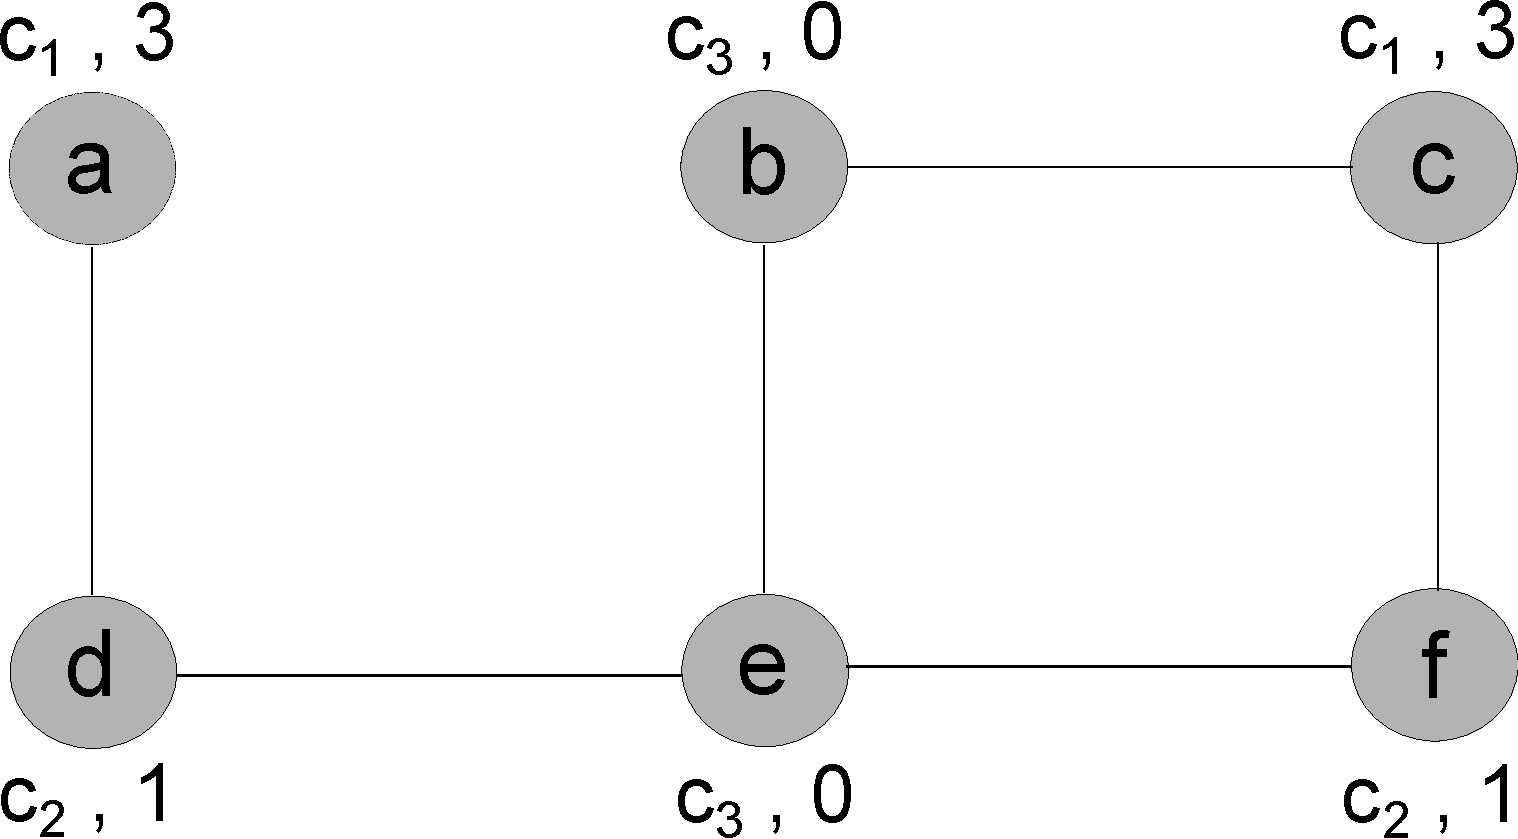
\includegraphics[width=0.3\textwidth]{figures/colors}
  \caption{ A hypothetical protein interaction network with six nodes
    \{a, b, c, d, e, f\}. The network is colored using three colors
    \{$c_1$, $c_2$, $c_3$\}. Each node carries two labels.  The label
    on the left denotes the color assigned to this node.  The one on
    the right is the node's $k_{max}$ value. For instance node d is
    assigned to color $c_2$ and its $k_{max}$ value is 1 (i.e., there
    is no other node assigned to color $c_2$ within 1-hop of node d). }
  \label{fig:colors}
\end{wrapfigure}


In this section, we build the mathematical model that will help us
compute the probability of success in each iteration.  Assume that we
are given a protein interaction network similar to the one described
in Section~\ref{introduction}, denoted by $G = (V, E, w)$, where $w(u,
v) = -$log $\lambda(u, v)$. Also assume that the colors of the nodes
are already assigned in the current iteration. We denote the set of
possible colors with $C = \{c_1, c_2, \ldots, c_m\}$ and the color of
node $v \in V$ with $c(v)$. We start by discuss several key concepts.


\begin{define} {\sc (Simple path)}
  Given a network $G=(V,E)$, a {\em simple path} from $u$ to $v$ ($u$,
  $v \in V$) is an ordering $<v_{1},v_{2}, \dots,v_{k}>$, of a subset
  of the vertices of $G$ such that $v_{1}=u$, $v_{k}=v$,
  $(v_{i},v_{i+1}) \in E$ and $v_i \neq v_j$ for all $i \neq j$.
\end{define}

Consider two nodes $u$ and $v$ in $G$. Let $k$ be a positive integer.
We say that $v$ is {\em reachable} from $u$ in $k$ hops if there is a
simple path from $u$ to $v$ that contains $k$ edges.

\begin{define}
  {\sc ($k$ neighborhood of a node)}. Let $v \in V$ be a node in $G$,
  and $k$ be a nonnegative integer.  We define the $k$ neighborhood of
  node $v$ as the set of nodes in $V \backslash \{v\}$ which are
  reachable from $v$ in $k$ hops of less. We denote this set using
  notation $\Psi_k(v)$.
\end{define}

Figure~\ref{fig:colors} shows an example of a colored network.  In
this example, $\Psi_1(a) = \{d\}$ because the node $d$ is the only
node that is reachable from the node $a$ in 1 hop (or less).
Similarly, $\Psi_1(f) = \{c, e\}$, $\Psi_2(a) = \{d, e\}$ and
$\Psi_2(f) = \{c, e, b, d\}$.  Following definition establishes the
relationship between each node of the network and the rest of the
network based on the colors assigned to all the nodes.

\begin{define}
  {\sc ($k_{max}$ value of a node)}. Let $v \in V$ be a node in $G$.
  The $k_{max}$ value of $v$, denoted with $k_{max}(v)$, is the
  maximal value of $k$ such that the $k$ neighborhood of $v$ does not
  contain a node with the same color as $v$. Formally, $ k_{max}(v) =
  \textrm{argmax}_k \{ \forall u \in \Psi_k(v), c(u) \neq c(v) \}.  $
\label{dfn:kmax:node}
\end{define}

Figure~\ref{fig:colors} shows the $k_{max}$ values for the nodes in
the network. For example, the colors of all the nodes in $\Psi_1(f) =
\{c, e\}$ are different than the color of $f$. When we expand the
neighborhood of $f$ by one, we get $\Psi_2(f) = \{c, e, b, d\}$. In
this set, $c(d) = c(f) = c_2$.  Therefore $k_{max}(f) = 1$.  Similarly
analysis shows that, $k_{max}(a) = 3$ and $k_{max}(b) = 0$. Next
definition characterizes a simple path of the network.

\begin{define} {\sc ($k_{max}$ configuration of a path)}.  Consider a
  simple path $\Phi = v_1 \rightarrow v_2 \rightarrow \ldots
  \rightarrow v_m$ of $m$ nodes in $G$. The $k_{max}$ configuration of
  $\Phi$ is the vector [$k_{max}(v_1)$, $k_{max}(v_2)$, $\ldots$,
  $k_{max}(v_m)$].
\end{define}

As an example, in Figure~\ref{fig:colors}, the $k_{max}$ configuration
of the path $\Phi = a \rightarrow d \rightarrow e \rightarrow f$ is
[3, 1, 0, 1]. That for $a \rightarrow d \rightarrow e \rightarrow b$ is
[3, 1, 0, 0].



\subsection{Bounding the probability of success tightly}
%\subsection{Bounding the number of colorings tightly}
\label{sec:bound}



In this section, we focus on one coloring iteration and describe how
we compute the probability of success in that iteration.
Consider any colorful path with $m$ nodes. The number of ways to
assign colors to the nodes of that path while keeping it colorful is
$m!$. Notice that this is equal to the numerator in Equation~\ref{ps}
for probability of success. The denominator in that equation, denoted
by $N_c$, is the total number of ways to color that path regardless of
whether it yields a colorful path or not. 

Notice that there can be many different color assignments that yield
the same $k_{max}$ configuration for the same path. Also, as we will
show later, the number of possible color assignments to the nodes of a
path can be different for different $k_{max}$ configurations. Indeed,
the $k_{max}$ configuration of a path describes the constraints
imposed on all the nodes of that path about how many alternative
colors can be assigned to them.  Following from this observation, we
first build a new undirected and unweighted graph, called the {\em
  constraint graph} from the $k_{max}$ configuration. By utilizing the
constraint graph we transform the problem of finding the number of
possible colorings to the chromatic polynomial computation problem.
Next, we describe how we build the constraint graph and how we utilize it to find the number of colorings.

\noindent
{\bf Building the constraint graph.}
Assume that we are given a simple path $\Phi = v_1 \rightarrow v_2
\rightarrow \ldots \rightarrow v_m$ of $m$ nodes along with its
$k_{max}$ configuration [$k_{max}(v_1)$, $k_{max}(v_2)$, $\ldots$,
$k_{max}(v_m)$]. We build a constraint graph with $m$ nodes \{$u_1$,
$u_2$, $\ldots$, $u_m$\}.  We denote the constraint graph as $G^{\Phi}
= (V^{\Phi}, E^{\Phi})$ where $V^{\Phi}$ is its set of nodes and
$E^{\Phi}$ is its set of edges.  For each pair of nodes $u_i$ and
$u_j$ in $V^{\Phi}$, we draw an undirected edge between them if the
following condition holds:
$$
j - i \leq \max\{k_{max}(v_i), k_{max}(v_j)\}.
$$

Notice that the indices $i$ and $j$ in the above description show the
positions of the nodes on the given path $\Phi$.  As a result, an edge
between $u_i$ and $u_j$ in the constraint graph indicates that $v_i$
and $v_j$ can not be of the same color according to the underlying
$k_{max}$ configuration. Thus, each possible coloring of the given
path $\Phi$ that obeys the $k_{max}$ configuration corresponds to a
chromatic coloring of the constraint graph $G^{\Phi}$ and vice versa.
Figure~\ref{maxk} shows an example of a path, its $k_{max}$
configuration and the corresponding constraint graph.


\begin{wrapfigure}{r}{0.350\textwidth}
%\begin{figure}[t]
\centering
\subfigure[]{
  \label{maxk:path}
  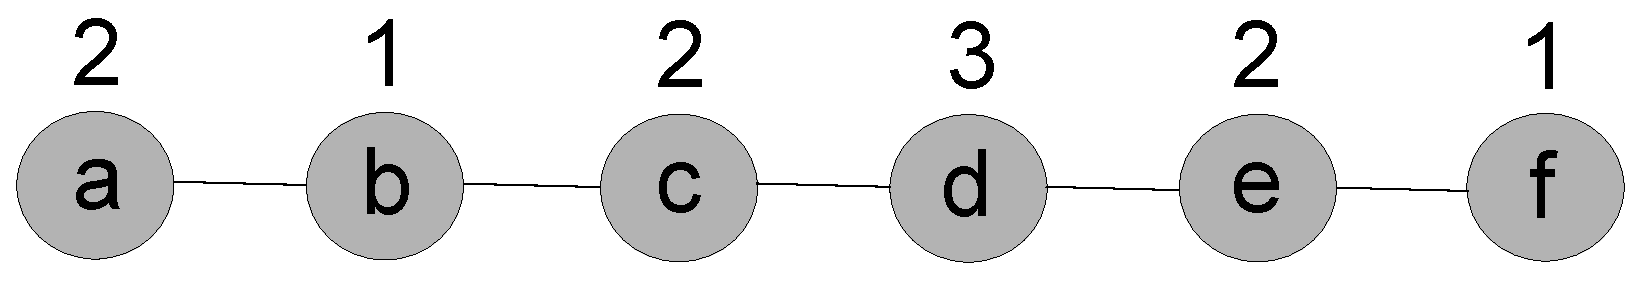
\includegraphics[width = 0.3\textwidth]{figures/kmax_path}
}
%\goodgap
\\
\subfigure[]{
  \label{maxk:graph}
  \includegraphics[width = 0.25\textwidth]{figures/kmax_graph}
}
\caption{(a) An example 6-node path with its $k_{max}$ configuration
  shown above it.  (b) The corresponding constraint graph $G^{\Phi}$.
}
  \label{maxk}
\end{wrapfigure}


\noindent
{\bf Computing the number of colorings.}
Formally, the value of the chromatic polynomial $A(G^{\Phi}, m)$ is
equal to the number of ways of coloring $G^{\Phi}$ using $m$ colors
without any pair of adjacent nodes having the same color.  Applying
chromatic polynomials on the constraint graph of a path yields the
number of possible colorings of that path.  We use a dynamic
programming solution following edge-contraction recursive rule based
on the fundamental reduction theorem~\cite{dong}.  To describe this,
we first define two contraction operators on graph $G^{\Phi}$. The
first one removes one edge, ($u$, $v$) from the edge set of
$G^{\Phi}$. We denote this with $G^{\Phi} - (u, v)$. The second one
merges two nodes, $u$ and $v$, into a single node $uv$. To do this, we
insert a new node $uv$ to $G^{\Phi}$. We also insert an edge between
$uv$ and all the nodes which are adjacent to either $u$ or $v$. We
then remove the nodes $u$ and $v$ along with all the edges incident to
them. We denote this merge operation with $G^{\Phi} / \{u, v\}$. Using
this notation, the chromatic polynomial is computed using the
following recurrence relation
\begin{equation}
A(G^{\Phi}, m) = A(G^{\Phi}- (u, v), m) - A(G^{\Phi} / \{u, v\}, m)
\label{eqchromatic}
\end{equation}
The stopping criteria in this recurrence is the case when $G^{\Phi}$ does not
contain any edge (i.e., no more constraints are remaining). In other
words $G^{\Phi} = (V^{\Phi}, \emptyset)$. In that case, all the nodes can take any
of the $m$ colors, and thus $A(G^{\Phi}, m) = m^{|V^{\Phi}|}$.  In
Equation~\ref{eqchromatic}, the first term, i.e, $A(G^{\Phi} - (u, v), m)$,
formulates the number of chromatic colorings by disregarding the
constraint between $u$ and $v$. The second term, i.e, $A(G^{\Phi} / \{u, v\},
m)$ corresponds to the number of colorings in which only the
constraint between $u$ and $v$ violates chromatic coloring of $G^{\Phi}$. So,
the difference of these two terms yields the number of chromatic colorings of $G^{\Phi}$.


Now we are ready to compute the probability of success, $P_s$, for a
coloring instance of our method (i.e, Step 6 of Algorithm~\ref{alg1}).
At each iteration, we first build the constraint graph $G^{\Phi}$ of the best
colorful path $\Phi$ found at that iteration. We compute the number of
chromatic colorings of $G^{\Phi}$ as $A(G^{\Phi}, m)$ as described above.  We then
set $N_c = A(G^{\Phi}, m)$ and compute the probability of success using
Equation~\ref{ps} as $P_s = m!/N_c = m!/A(G^{\Phi}, m)$.


\subsection{Analysis of the probability of success}
\label{sec:theory}


One key question would regarding how we compute the probability of
success is: Is it guaranteed to be better than existing methods
including Scott {\it et al.}~\cite{scott} and G{\"u}lsoy {\it et
  al.}~\cite{gulsoy}? In this section, we answer this theoretically.
We start by defining a partial order between $k_{max}$ configuration
of a paths as follows: Consider two such configurations ${\bf x} =$
[$x_1$, $x_2$, $\ldots$, $x_m$] and ${\bf y} =$ [$y_1$, $y_2$,
$\ldots$, $y_m$]. We say that ${\bf x} \leq {\bf y}$ if and only if
$\forall_i$, $x_i \leq y_i$.


\begin{proposition}
  Consider two $k_{max}$ configurations ${\bf x}$ and ${\bf y}$ of two
  simple paths each having $m$ nodes. Let us denote their
  corresponding constraint graphs $G_x$ and $G_y$ respectively. If
  ${\bf x} \leq {\bf y}$ then $A(G_x, m) \geq A(G_y, m)$.
\label{prop:order}
\end{proposition}

We ommit detailed proof of Proposition~\ref{prop:order} due to space
limitation. However, briefly it follows from the observation that
${\bf x} \leq {\bf y}$ implies that every edge in $G_x$ also appears
in $G_y$. However, the opposite may not be true. In other words, $G_x$
has only a subset of the constraints imposed by $G_y$. Thus, the
chromatic polynomial $A(G_x, m)$ cannot be less than $A(G_y, m)$.

Proposition~\ref{prop:order} has two important implications. First,
traditional color coding method (such as Scott {\it et al.}~\cite{scott})
computes $N_c = m^m$. This is the most conservative case in our model
when the $k_{max}$ configuration is [0, $\ldots$, 0].  Clearly, this
will yield the worst (i.e., largest) possible value for the chromatic
polynomial since $[0, $\ldots$, 0] \leq {\bf y}$ for any $k_{max}$
configuration ${\bf y}$. Second, let $t$ be the smallest $k_{max}$
value among all the nodes in the network. The formulation by
G{\"u}lsoy {\it et al.}~\cite{gulsoy} corresponds to $k_{max}$ configuration
is [$t$, $\ldots$, $t$]. Let ${\bf y}$ be the $k_{max}$ configuration
of any $m$-node path in the same network. We have [$t$, $\ldots$, $t$]
$\leq {\bf y}$ since all the entries of ${\bf y}$ have value $t$ or
more.  {\em We conclude from these two implications that our method is
  guaranteed to produce less or same $N_c$ value as the mentioned
  existing methods depending on the network topology and the color
  distribution.  Smaller values for $N_c$ implies larger success
  probability, and thus, faster convergence to the desired confidence
  value.}



As an example, our method computes the value of $N_c$ for the path
shown in Figure~\ref{maxk:path} is 5,760, while Scott {\it et
al.}~\cite{scott} and G{\"u}lsoy {\it et al.}~\cite{gulsoy} yield $N_c$ =
46,656 and 18,750 respectively for the same example.  According to
Equation~\ref{ps}, such a decrease in the value of $N_c$ leads 8.1 and
3.2 times larger success probability than the two above-mentioned
methods respectively.


\ignoreme{

\tk{Maybe we should not include the blue stuff below.}

{\color {blue}

To answer the second question, we need to focus on the path that
provides the $k_{max}$ configuration for computing $N_c$. Ideally, the
$k_{max}$ configuration should be obtained from the path with the
smallest weight. This is however impossible since that is actually the
path we are trying to find. Instead, we are using the smallest
weighted path among the colorful paths. Thus, the $N_c$ value we
compute may be different than the true $N_c$ value. That said, it is
also worth noting that the true $N_c$ value is among appears in the
distribution of possible $N_c$ values since it is possible to assign
colors so that the smallest weighted path is colorful. Our computation
may over or under estimate the $N_c$ value at an iteration. If we over
estimate it, it will not affect the correctness of our algorithm. This
is because large $N_c$ values will only impose more iterations than
necessary leading to lower performance but true result.  If we under
estimate $N_c$, that will increase the confidence value more than
necessary. This may lead to early termination of the iterations. 



The confidence value in Algorithm~\ref{alg1} (i.e., $P$ in Step 7) is
a product of failure probabilities.  To understand how well our
estimation is, we focus on the distribution of the $N_c$ estimations
done throughout iterations. Since the color assignments at different
iterations are independent, we know that the $N_c$ estimates are
independent and identically distributed (iid).  From central limit
theorem, we know that the mean and of a population of iid samples
quickly converges to normal distribution.  Let us denote the random
variable that produces $1- m!/N_c$ at the $i$th coloring iteration
with $X_i$.  Thus, after $t$ iterations, $\log(1-P) / t$ is simply the
mean of the population with samples being $Y_i = \log X_i$. This
provides us a systematic way to control the amount of error that can
be introduced. By moving away from the mean we can precisely tell the
probability that our confidence is an over or under estimate of the
true confidence. We defer further discussion to experimental results.
}

}

%
\section{Experiments}
\label{sec:exp}

In this section, we evaluate our method on real datasets. We
implemented our method in Java language. We ran our experiments on Java
runtime environment version 1.6 on Linux machines with 2.2-GHz dual AMD Opteron
dual core processors, and 3 GBs of main memory.

\paragraph{Datasets}
In our experiments, we used two datasets of protein interactions
in Homo Sapiens and Rattus Norvegicus from MINT\cite{mint1} (the Molecular
INTeraction database). The first one is a large dataset of 15472 interactions
among 6122 proteins. The second one is a smaller dataset of 806 interactions
among 631 proteins. Each interaction is described by two interacting proteins and a
reliability score between 0 and 1 that represents the level of confidence that
this interaction truly exists. MINT calculates reliability scores of
interactions using a heuristic formula of available evidence, including the
size and type of the experiment reporting the interaction, sequence similarity
of ortholog proteins and the number of publications supporting the
interaction\cite{mint2}. 

We use the negative logarithm of MINT reliability scores as edge weights. In all
experiments, we find pathways starting within the set of membrane proteins and
ending within the set of transcription factors. We use the Gene Ontology
database\cite{go} to identify membrane proteins and transcription factors of each
dataset. We identify membrane proteins as the ones under the terms GO:0005886
and GO:0004872, and transcription factors as the proteins under the terms
GO:0000988, GO:0001071 and GO:0006351.

\subsection{Performance assessment and comparison}


\begin{figure}[h]
\centering
\subfigure[H.sapiens, path length = 6]{
	\label{iterations_hsa_6}
	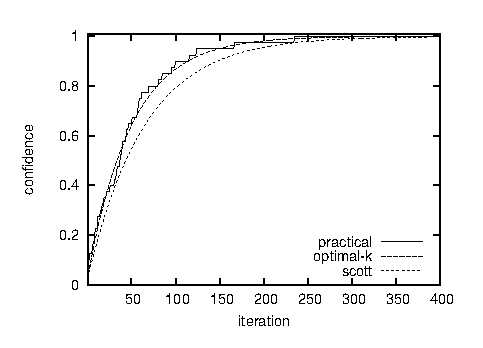
\includegraphics{results/iterations/hsa6}
}
\goodgap
\subfigure[H.sapiens, path length = 8]{
	\label{iterations_hsa_8}
	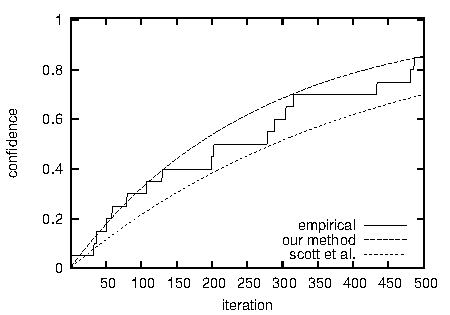
\includegraphics{results/iterations/hsa8}
}
\subfigure[R.norvegicus, path length = 6]{
	\label{iterations_rat_6}
	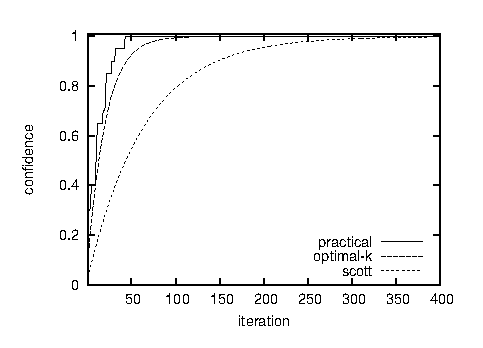
\includegraphics{results/iterations/rat6}
}
\goodgap
\subfigure[R.norvegicus, path length = 8]{
	\label{iterations_rat_8}
	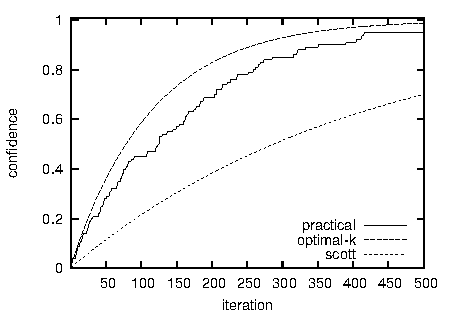
\includegraphics{results/iterations/rat8}
}
\caption{Confidence level acheived after a given number of iterations,
comparing our method to Scott et al. and empirical confidence. X-axis is the
number of iterations finished, and Y-axis is the level of confidence in the
optimality of the result, for H.sapiens and R.norvegicus at different path
lengths. The empirical line denotes the observed probability that the optimal
path is found at or before a given iteration, averaged over several experiments.}
\label{iterations}
\end{figure}



We run an experiment to measure how fast the value of confidence rises with each
iteration in both our method and the one presented by Scott et al.\cite{scott}.
We run each method for 500 iterations and measure the overall confidence after
each iteration is finished. We also compare these results with the empirical
confidence, which is the probability of finding the optimal pathway as
empirically observed. To compute the empirical confidence, we run 500
coloring iterations and assign each iteration a value $s \in \{0, 1\}$, where
$s = 1$ if the optimal pathway is found in this iteration or in a preceding one,
and $s = 0$ otherwise. We repeat this experiment multiple times and take the
average values of $s$ for each iteration as the empirical confidence of this
iteration. Figure \ref{iterations} shows the confidence value as more iterations
finish, for our method and Scott et al. and also the empirical confidence value.
The figure shows a gap between Scott et al. confidence and empirical confidence,
which is expected because of the conservative way they use to calculate success
probability of an iteration, as discussed in section \ref{background}. This gap
increases as the path length parameter increases. Our method closes this gap and
produces confidence values that are closer to the empirical confidence values.
The figure also shows that our method produces higher confidence values than
Scott et al. for the same number of iterations.

\begin{figure}[h]
\centering
\subfigure[H.sapiens, path length = 6]{
	\label{times_hsa_6}
	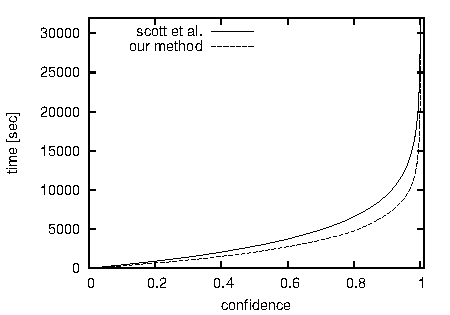
\includegraphics{results/times/time_hsa6}
}
\goodgap
\subfigure[H.sapiens, path length = 8]{
	\label{times_hsa_8}
	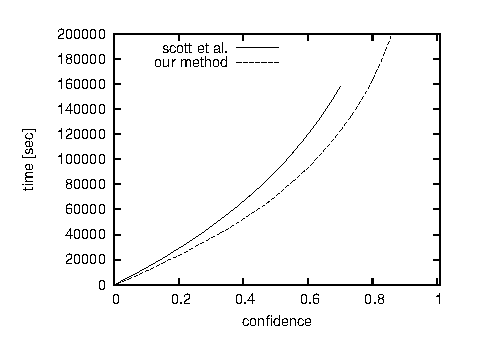
\includegraphics{results/times/time_hsa8}
}
\subfigure[R.norvegicus, path length = 6]{
	\label{times_rat_6}
	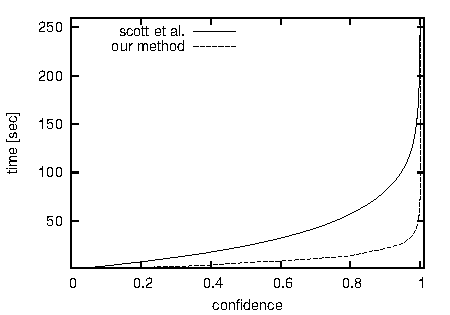
\includegraphics{results/times/time_rat6}
}
\goodgap
\subfigure[R.norvegicus, path length = 8]{
	\label{times_rat_8}
	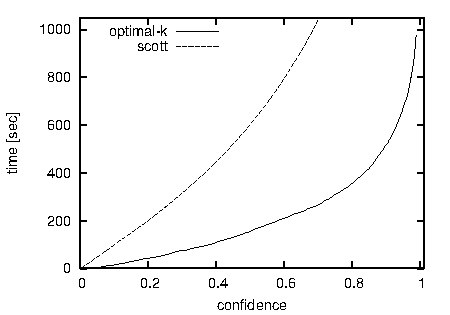
\includegraphics{results/times/time_rat8}
}
\subfigure[R.norvegicus, path length = 9]{
	\label{times_rat_9}
	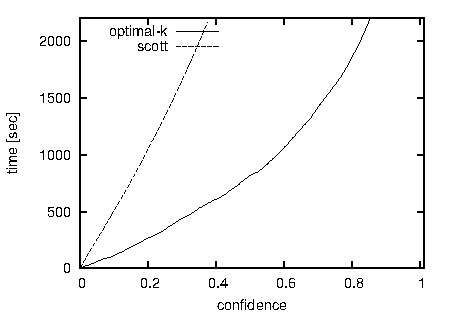
\includegraphics{results/times/time_rat9}
}
\caption{Total time needed to acheive a given level of confidence by our method
and Scott et al. X-axis is the level of confidence in the optimality of the
result, and Y-axis is the total time taken to acheive this confidence level,
for H.sapiens and R.norvegicus at different path lengths. Lower values are
better.}
\label{times}
\end{figure}



We also measure the total time taken by our method to reach a given
confidence level as opposed to that of Scott {\it et
  al.}~\cite{scott}. We run both methods for 500 iterations and
measure, after each iteration, the confidence level reached and the
overall time taken by both methods. Figure \ref{times} shows that our
method takes less time than Scott et al. to achieve the same level of
confidence. The figure also shows that the our performance lead
increases as the path length parameter increases.



\subsection{Validation Experiments}
\label{sec:validation}


So far we have shown that our method outperforms existing coloring
strategies in terms of the running time performance. In this section,
we evaluate the biological significance of the results we can find
using our method. 

It is worth mentioning that our method returns the same results as
Scott {\it et al.}~\cite{scott} when both of them are allowed to reach
a high confidence value (such as 99\% confidence). The main difference
is that our method scales to larger networks and longer paths.
Therefore, here we will only focus on the results obtained by our
method.


\subsubsection{Statistical significance of the results}
\label{sec:zscore}

%\begin{wraptable}{r}{0.40\textwidth}
\begin{table}[t]
  \tbl{$Z$-scores calculated for the optimal paths found by our method for
  H.sapiens and R.norvegicus for different path lengths. $Z = \frac{\mu
  - \theta}{\sigma}$ where $\mu$ is the average weight of 1000 randomly
  generated paths, $\sigma$ is their standard deviation, and $\theta$ is the
  weight of the optimal path found by our method.} {
\begin{tabular}{|l|c|c|c|c|c|c|c|c|c|}
\hline
	&	\multicolumn{9}{c|}{Path Length}		\\ \cline{2-10}
Dataset	&	\multicolumn{3}{c|}{6}	&	\multicolumn{3}{c|}{7}	&
	\multicolumn{3}{c|}{8}	\\
	\cline{2-10} 
		&	\begin{math}\mu\end{math}	&	\begin{math}\theta\end{math}	&
	\begin{math}Z\end{math} & \begin{math}\mu\end{math}	&	\begin{math}\theta\end{math}	&
	\begin{math}Z\end{math} & \begin{math}\mu\end{math}	&
	\begin{math}\theta\end{math}	& \begin{math}Z\end{math}	\\ \hline
{\it H.sapiens}	&	5.906	&	0.129	&	5.409	&	7.074	&	0.130	&	5.477	&	8.341	&
0.221	&	5.764	\\
{\it R.norvegicus}	&	4.975	&	4.540	&	0.889	&	7.307	&	5.025	&	1.453	&
8.457	&	4.858	&	1.467
\\
\hline
\end{tabular}
}
\label{tab:zscore}
\end{table}
%\end{wraptable}

In this section we assess the statistical significance of the paths found of our
method; how our results compare to random paths. We use $Z$-score to
measure statistical significance. For each dataset and path length, we run our method to
get the path with the minimum weight $\theta$. we then generate 1000 random
simple paths that start at a membrane protein and end at a transcription
factor. We compute the average weight $\mu$ of these random paths and their
standard deviation $\sigma$. We then compute the $Z$-score as follows
\begin{equation}
Z = \frac{\mu - \theta}{\sigma}
\end{equation}
$Z$-score indicates by how many standard deviations our optimal weight is
better than the weight of an average random path, so higher values are better.
Table~\ref{tab:zscore} shows $Z$-scores for H.sapiens and R.norvegicus for path
length 6, 7 and 8. Our results are always better than the random ones.
The calculated $Z$-scores range from 0.89 to 5.76. It can also be observed that,
for a given dataset, $Z$-score increases with increasing the path length, which
is expected because increasing the size of random selection leads to less
chances of the selected path being better or closer to the optimal path.
From these observations observations, we can infer that our results are
statistically significant.


\subsubsection{Biological significance of the results}

\begin{wrapfigure}{r}{0.50\textwidth}
  \centering
  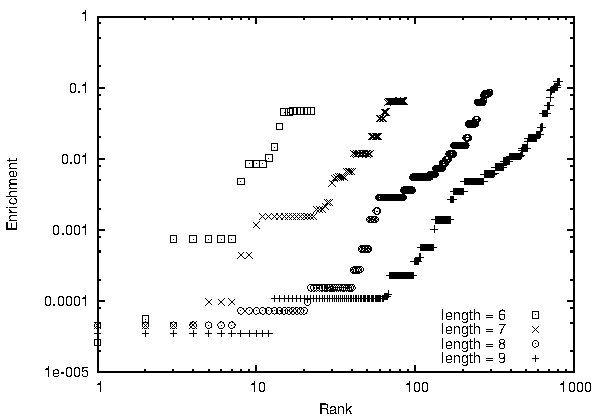
\includegraphics[width=0.45\textwidth]{results/enrichment/enrich-rank}
  \caption{Sorted values of functional enrichment of optimal and suboptimal
  paths found at different iterations of our method. X-axis is the rank of the
  path with regard to its functional enrichment in log scale, and Y-axis is the
  enrichment value of this path. Lower values are better.}
  \label{fig:enrichment-rank}
\end{wrapfigure}


\begin{wrapfigure}{r}{0.50\textwidth}
  \centering
  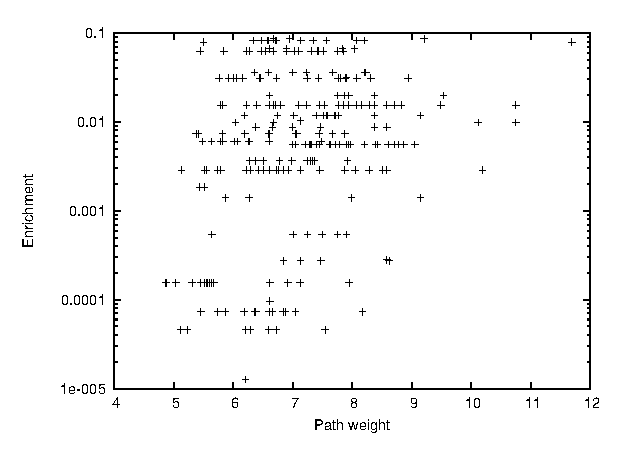
\includegraphics[width=0.45\textwidth]{results/enrichment/enrich-score}
  \caption{Functional enrichment values of paths against their weights. X-axis
  is path's weight and Y-axis is its corresponding enrichment value. Lower
  values are better.}
  \label{fig:enrichment-score}
\end{wrapfigure}


Another important question is: how biologically significant are our results? To
answer this question, we validate our results using functional enrichment. We
use the Gene Ontology\cite{go} to compute functional enrichment of paths found
at different iterations of our method. Let $\Phi$ be the path being tested, $T$
be the universal set of GO terms, $m$ be the path length, $M$ be the total
number of proteins in the dataset, $G_i$ be the total number of proteins
annotated with the Go term $t_i$ in the dataset, and $g_i$ be the number of
proteins annotated with $t_i$ in $\Phi$. We compute functional enrichment of
$\Phi$ as $\min_{t_i \in T} P(X \geq g_i | M, m, G_i)$ where $X$ is a random
variable under under a hypergeometric distribution with these parameters. Lower
values of are better.



 
\subsection{Discussing paths found}
 
 \begin{figure}[h]
\centering
\subfigure[All proteins annotated by GO:0042058 - regulation of epidermal growth
factor receptor signaling pathway]{
	\label{fig:path_go0042058}
	\includegraphics[width = 0.8\textwidth]{figures/path_go0042058}
}
\subfigure[First five proteins annotated by GO:0042059 - negative regulation of
epidermal growth factor receptor signaling pathway]{
	\label{fig:path_go0042059}
	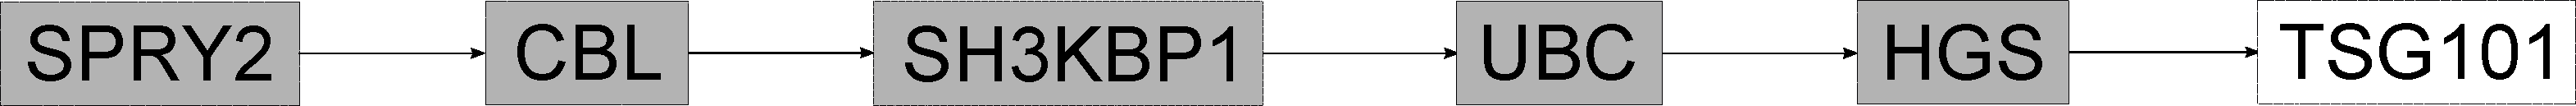
\includegraphics[width = 0.8\textwidth]{figures/path_go0042059_2}
}
\subfigure[All proteins annotated by GO:0046875 - ephrin receptor binding]{
	\label{fig:path_go0046875}
	
\includegraphics[width = 0.8\textwidth]{figures/path_go0046875}
}
\caption{Caption goes here}
\label{fig:paths}
\end{figure}
 



\section{Experiments}
\label{sec:exp}

In this section, we evaluate our method on real protein interaction
networks. We implemented our method in Java. We ran our experiments on
Linux machines with 2.2-GHz dual AMD Opteron dual core processors and
3 GBs of main memory.

\paragraph{Datasets}
We used the protein interactions of {\it H. sapiens} and {\it R.
  norvegicus} taken from the MINT database~\cite{mint1}. The first one
is a large dataset of 15,472 interactions among 6,122 proteins. The
second one is a smaller dataset containing 806 interactions among 631
proteins. Each interaction is described by two interacting proteins
and a reliability score between 0 and 1 that represents the level of
confidence that this interaction exists.  MINT calculates reliability
scores of interactions from available evidence, such as the size and
type of the experiment reporting the interaction, sequence similarity
of ortholog proteins~\cite{mint2}.

We use the negative logarithm of MINT reliability scores as edge
weights. In all experiments, we find pathways starting within the set
of membrane proteins and ending within the set of transcription
factors. We use the Gene Ontology database~\cite{go} to identify these
setes. We identify membrane proteins as the ones annotated with the
terms GO:0005886 and GO:0004872, and transcription factors as those
with GO:0000988, GO:0001071 and GO:0006351.

\subsection{Performance assessment}



\begin{figure}[t]
  \centering \subfigure[{\it H.sapiens}]{
	\label{times_hsa_8}
	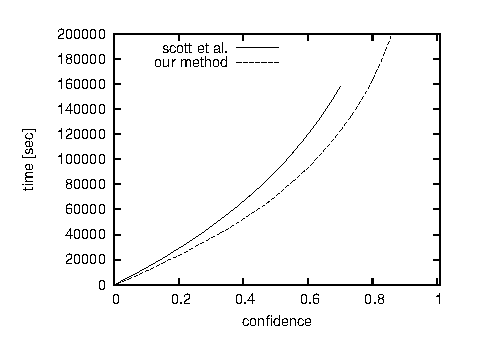
\includegraphics[width = 0.4\textwidth]{results/times/time_hsa8}
}
\goodgap
\subfigure[{\it R.norvegicus}]{
	\label{times_rat_8}
	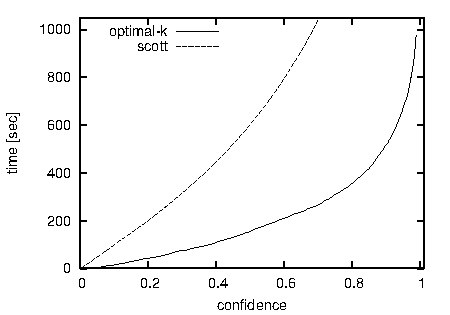
\includegraphics[width = 0.4\textwidth]{results/times/time_rat8}
}

\caption{Total time needed to acheive a given level of confidence by
  our method and Scott {\it et al.}  for {\it H.sapiens} and {\it
    R.norvegicus} for path length = 8.  }
\label{times}
\end{figure}

In Section~\ref{sec:theory}, we have already shown theoretically that
our method is guaranteed to be at least as fast as the traditional
color coding methods. The gap however depends on the topology of the
underlying protein interaction network. In this section, we
experimentally evaluate how the performance of our method compares to
Scott {\it et al.}~\cite{scott} as a leading method. We run both
methods on our datasets for 500 iterations. We repeat this experiment
for each of the pathway lengths = \{4, 5, 6, 7, 8, 9\}.  We measure
the total time taken and the confidence value computed by each method
at each iteration. We run this process multiple times (at least 20
times) and report the average of these runs. Below, we report a small
subset of these experiments due to page limits.


Figure~\ref{times} shows the time it takes to reach to various
confidence levels for path length = 8.  Our method takes much less
time than Scott {\it et al.}  to achieve the same level of confidence.
The gap between the two increases as the confidence level increases.
We observe that the gap is significantly larger for the {\it R.
  norvegicus} dataset. This is mainly because this dataset is more
sparse than the other one. As a result, it often produces very dense
constraint graphs leading to high success probability values.  Scott
{\it et al.} is, on the other hand, oblivious to the density of the
network. It produces the same conservative success probability for
both datasets. As a result, as we can see in Figure~\ref{times}, Scott
{\it et al.} can only reach to around 70\% confidence for both
datasets after 500 iterations. Our method, on the other hand, reports
85\% and more than 99\% confidence for the {\it H.  sapiens} and {\it
  R.  norvegicus} datasets respectively after the same number of
iterations. The difference between the largest confidence we report
for the two datasets can be explained from the density of the two
networks. As the network gets sparser, our method tends to gets larger
confidence value.  In Figure~\ref{times_hsa_8}, we see that our method
takes more time to complete 500 iterations than Scott {\it et al.}
This is because it spends additional time to build constraint graph
and solve a chromatic polynomial problem. Finally, we observed similar
characteristics for other path lengths (results not shown). The main
difference was that the performance gap between our method and Scott
{\it et al.} further increases with larger path lengths.


\begin{figure}[t]
\centering
\subfigure[{\it H.sapiens}]{
	\label{iterations_hsa_6}
	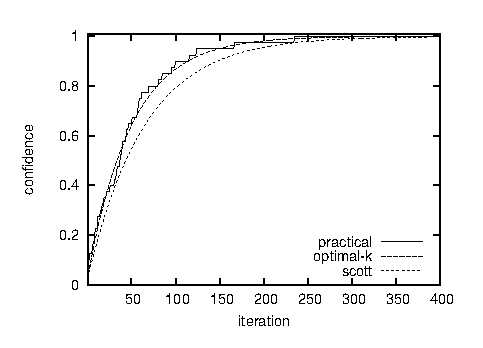
\includegraphics[width = 0.4\textwidth]{results/iterations/hsa6}
}
\goodgap
\subfigure[{\it R.norvegicus}]{
	\label{iterations_rat_6}
	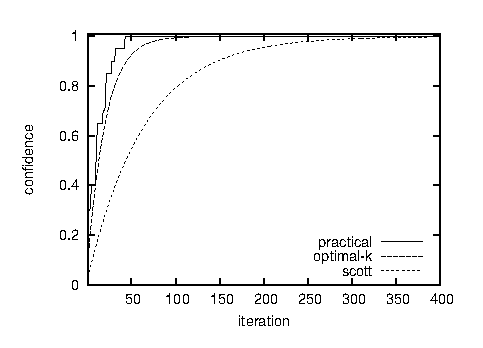
\includegraphics[width = 0.4\textwidth]{results/iterations/rat6}
}
\caption{Confidence level acheived after a given number of iterations
  using our method and to Scott {\it et al.}~\cite{} for {\it H.sapiens} and
  {\it R.norvegicus} when path length is fixed at 6. Empirical results
  denote the fraction of experiments in which the optimal path is
  found at or before a given iteration.}
\label{iterations}
\end{figure}

In our next experiment, we evaluate whether our confidence computation
is correct in practice.  To do this, we computed an empirical
confidence as follows.  Recall that we repeated each experiment many
times.  At each iteration we computed the fraction of the experiments
in which we were able to find the optimal result as the empirical
confidence.  Ideally, the theoretical value should not be larger than
the empirical one; the closer the two values are the better.
Figure~\ref{iterations} shows the empirical confidence value as well
as the theoretical confidence value of our method and Scott {\it et
  al.}.  The results demonstrate that the gap between the empirical
results and our method is much smaller than that for Scott {\it et
  al.}  This is because of the conservative way they use to calculate
success probability of an iteration as discussed in
section~\ref{sec:back}.  This gap increases as the path length
parameter increases (results not shown).  Thus, we conclude that both
Scott {\it et al.} and our method produces correct confidence values.
Scott {\it et al.} is, however to conservative, and thus spends too
many iterations to reach to the same confidence value.


\subsection{Validation Experiments}
\label{sec:validation}


So far we have shown that our method outperforms existing coloring
strategies in terms of the running time performance. In this section,
we evaluate the biological significance of the paths found using our
method.  It is worth mentioning that our method returns the same
results as Scott {\it et al.}~\cite{scott} when both of them are
allowed to reach a high confidence value (such as 99\% confidence).
The main difference is that our method scales to larger networks and
longer paths.  Therefore, here we will only focus on the results
obtained by our method.


\subsubsection{Statistical significance of the results}
\label{sec:zscore}

%\begin{wraptable}{r}{0.40\textwidth}
\begin{table}[t]
  \tbl{$Z$-scores calculated for the optimal paths found by our method for
    {\it H.sapiens} and {\it R.norvegicus} for different path lengths. 
    Here, $\mu$ is the mean  of the 
    weight of a  random path in the same network with the same length.
    $\theta$ is the
    weight of the optimal path found by our method. $Z$ is the 
    Z-score of our method.} {
\begin{tabular}{|l|c|c|c|c|c|c|c|c|c|}
\hline
	&	\multicolumn{9}{c|}{Path Length}		\\ \cline{2-10}
Dataset	&	\multicolumn{3}{c|}{6}	&	\multicolumn{3}{c|}{7}	&
	\multicolumn{3}{c|}{8}	\\
	\cline{2-10} 
		&	\begin{math}\mu\end{math}	&	\begin{math}\theta\end{math}	&
	\begin{math}Z\end{math} & \begin{math}\mu\end{math}	&	\begin{math}\theta\end{math}	&
	\begin{math}Z\end{math} & \begin{math}\mu\end{math}	&
	\begin{math}\theta\end{math}	& \begin{math}Z\end{math}	\\ \hline
{\it H.sapiens}	&	5.906	&	0.129	&	5.409	&	7.074	&	0.130	&	5.477	&	8.341	&
0.221	&	5.764	\\
{\it R.norvegicus}	&	4.975	&	4.540	&	0.889	&	7.307	&	5.025	&	1.453	&
8.457	&	4.858	&	1.467
\\
\hline
\end{tabular}
}
\label{tab:zscore}
\end{table}
%\end{wraptable}


In this section we assess the statistical significance of the paths
found of our method. We use $Z$-score to measure statistical
significance. $Z$-score indicates by how many standard deviations our
optimal weight is better than the weight of an average random path, so
higher values are better. For each dataset and path length, we run our
method to get the path with the minimum weight $\theta$. We then
generate 1000 random simple paths of the same length as that found by
our method, starting at a membrane protein and ending at a
transcription factor.  We compute the average weight $\mu$ of these
random paths and their standard deviation $\sigma$. We then compute
the $Z$-score as $Z = \frac{\mu - \theta}{\sigma}$.


Table~\ref{tab:zscore} shows the results for {\it H.sapiens} and {\it
  R.norvegicus} for path lengths 6, 7 and 8. Our results are always
better than the random paths.  Particularly, for the {\it H.sapiens}
network we obtain very significant results. The $Z$-score for {\it
  R.norvegicus} is less. This is mainly because the edge confidence
values in this network have much less variation than those in {\it
  H.sapiens}.  Our $Z$-score increases with increasing path length.
This is not surprising because increasing the size of random selection
leads to less chances of the selected path being better or closer to
the optimal path.  This implies that there is a great potential that
methods that scale to large path length will yieled important
biological insights into signaling pathway identification.

\subsubsection{Biological significance of the results}


\begin{wrapfigure}{r}{0.450\textwidth}
  \centering
  \vspace*{-1.5cm}
  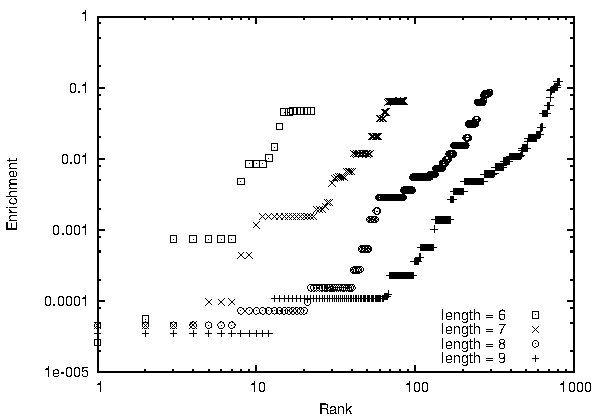
\includegraphics[width=0.4\textwidth]{results/enrichment/enrich-rank}
  \caption{Functional enrichment of best colorful paths found at
    different iterations of our method for {\it R.norvegicus} in
    sorted order. Smaller values are better.}
  \label{fig:enrichment-rank}
\end{wrapfigure}


Another important question is: how biologically significant are our
results? To answer this question, we validate our results using
functional enrichment. We use the Gene Ontology~\cite{go} to compute
functional enrichment of paths found at different iterations of our
method. Let $\Phi$ be the path being tested, $T$ be the universal set
of GO terms, $m$ be the path length, $M$ be the total number of
proteins in the dataset, $G_i$ be the total number of proteins
annotated with the Go term $t_i$ in the dataset, and $g_i$ be the
number of proteins annotated with $t_i$ in $\Phi$. We compute
functional enrichment of $\Phi$ as $\min_{t_i \in T} P(X \geq g_i | M,
m, G_i)$ where $X$ is a random variable under a hypergeometric
distribution with these parameters. Lower enrichment values indicate
paths with common functions, and thus they are better.

\begin{wrapfigure}{r}{0.50\textwidth}
%\begin{figure}[h]
  \centering
  \subfigure[]{
  \label{fig:path_go0042058}
  \includegraphics[width = 0.45\textwidth]{figures/path_go0042058}
} \\


\subfigure[]{
  \label{fig:path_go0046875}
  
\includegraphics[width = 0.45\textwidth]{figures/path_go0046875}
} \\

\subfigure[]{
  \label{fig:path_go0042059}
  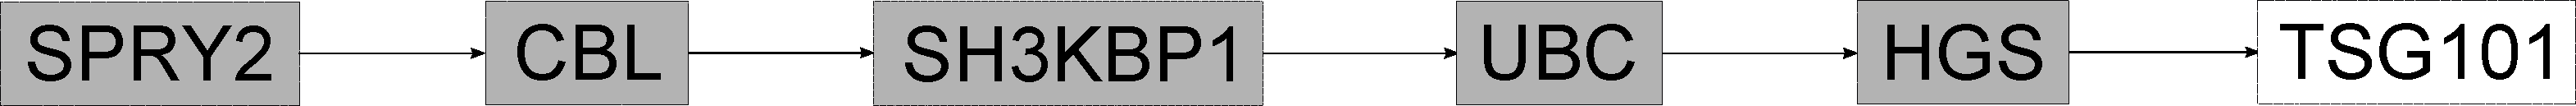
\includegraphics[width = 0.45\textwidth]{figures/path_go0042059_2}
} 

\caption{Three sample pathways with functional enrichment value less
  than $10^{-11}$ found by our method in the {\it H.sapiens} dataset. The shaded nodes correspond
  to the genes which have commong gene ontology term.  (a) The common
  term is GO:0042058 (c) The common term is GO:0042059 - negative
  regulation of epidermal growth factor receptor signaling pathway (b)
  The common term is GO:0046875 - ephrin receptor binding }
\label{fig:paths}
\end{wrapfigure}


Figure~\ref{fig:enrichment-rank} plots the functional enrichment value
of the best colorful paths found at different iterations of our
algorithm in sorted order for the {\it R.norvegicus} network. We omit
results for {\it H. sapiens} as it is very similar to those in
Figure~\ref{fig:enrichment-rank}.  We observe that as the distribution
of the enrichment values follows power-law distribution. That is only
a minority of the observed paths have very good enrichment while the
majority tend to have bad ones. We observe that this behavior is
consistent for all path lengths we tested. This suggests the
following: (i) There can be multiple biologically interesting paths
for the same start and end node sets.  (ii) We need to have
sufficiently high confidence in the result to avoid biologically
meaningless paths since the enrichment drops quickly.  (iii) Even long
paths can be highly enriched. All of these observations show the
importance of improving the running time performance of pathway
discovery methods, and hence the importance of our contribution in
this paper.

\ignoreme{

\tk{I am commenting out this result to save space}

\begin{wrapfigure}{r}{0.450\textwidth}
  \centering
  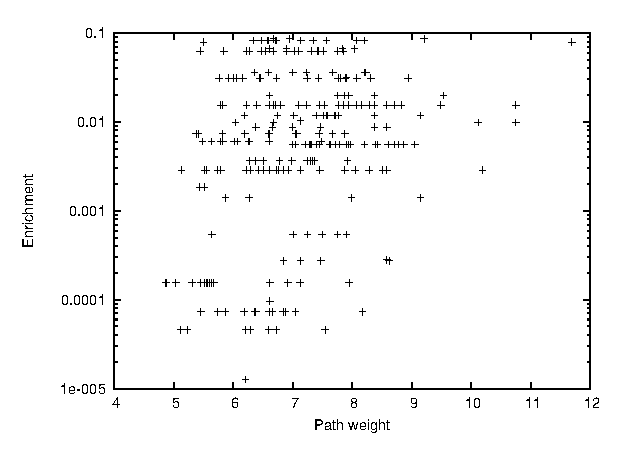
\includegraphics[width=0.4\textwidth]{results/enrichment/enrich-score}
  \caption{Functional enrichment values of best colorful eight node
    paths reported at different iterations against their weights for
    {\it R.norvegicus}. }
  \label{fig:enrichment-score}
\end{wrapfigure}



Figure~\ref{fig:enrichment-score} shows the relation between a path
weight and its enrichment value. While the relation is not clear-cut
for paths with relatively low weights, it is evident that paths with
higher weights tend to have bad enrichment values. This observation
backs the need to explore paths with lower weights, and shows the
value in finding paths in ascending order of their weights.
Figure~\ref{fig:enrichment-rank} and figure~\ref{fig:enrichment-score}
also show that all the discovered paths have enrichment values ranging
from $0.1$ to $10^{-5}$, which is a very good range of enrichment
values for the discovered paths that shows that our results are
biologically significant.
}


 
Next, we focus on a few of the most functionally enriched pathways our
method finds on the {\it H. sapiens} network.  Figure~\ref{fig:paths}
shows three examples each having length of six. All the six genes in
the path in Figure~\ref{fig:path_go0042058} regulate epidermal growth
factor receptor signaling pathway.  Among these the leftmost four
genes appear in the ErbB signaling pathway.  They also affect the
development of various cancer types such as chronic myeloid leukemia,
glioma and prostate cancer.  In Figure~\ref{fig:path_go0046875}, all
the six genes are ephrin receptor binding. They affect cell growth and
development and thus participate in cancer development.  The five
leftmost genes in Figure~\ref{fig:path_go0042059} negatively regulate
the epidermal growth factor receptor signaling pathway.  Notice that
all the three pathways in this example overlap with each other, yet
they also contain several genes that do not exist in others.  For
instance, the pathway in Figure~\ref{fig:path_go0046875} contains SRC
unlike the other. SRC takes part in same pathways as most of the other
genes in this figure, such as the ErbB signaling pathway.  Thus, all
of these significant paths reported by our method reveal different
parts of the signaling networks through alternative paths.



\section{Conclusion}
\label{sec:conc}

{\small
In this paper, we presented an enhanced color-coding technique. We presented a
novel way to calculate success probability for a single coloring iteration. We
explained how to calculate the number of coloring possibilities for a path
with a given $k_{max}$ configuration. We also discussed the relation between
configurations with different $k_{max}$ values. We used the enhanced
color-coding technique to find signaling pathways in protein interaction
networks. We empirically showed that our method produces correct results, and
that it needs less time than the leading method to produce these results. We
also showed that the results of our method are of statistical and biological
significance.}

\bibliographystyle{ws-procs11x85}
\bibliography{references}


\end{document}